\chapter{Exploratory Data Analysis}

\section{Data Structure and Overview}
The Knuth Miles dataset is structured as a complete weighted undirected graph with the following characteristics:
\begin{itemize}
    \item Number of nodes (cities): 128
    \item Number of edges (connections): 8128
    \item Edge weights: Distances in miles between cities
    \item Node attributes: City name, coordinates, and population
\end{itemize}

\section{Data Export Process}
The data was processed and exported into two main files:

\subsection{Node Data Export}
The city nodes data was exported to \texttt{Node\_cities.csv} with the following structure:
\begin{itemize}
    \item City name
    \item Longitude
    \item Latitude
    \item Population (in thousands)
\end{itemize}

\subsection{Edge Data Export}
The edge data was exported to \texttt{edges.csv} containing:
\begin{itemize}
    \item Source city
    \item Target city
    \item Distance weight
\end{itemize}

\section{Data Quality Analysis}
The dataset exhibits the following characteristics:
\begin{itemize}
    \item No missing values in the distance measurements
    \item Complete graph structure (all cities connected to all others)
    \item Population data ranges from 3,000 to 876,000
\end{itemize}

\section{Geographic Distribution Analysis}
The geographic distribution of cities reveals several key patterns:

\subsection{City Clustering}
\begin{itemize}
    \item Dense clusters in the Northeast and Midwest regions
    \item Sparse connections in the Western and Southern regions
    \item Natural geographical barriers influencing connectivity
\end{itemize}

\subsection{Geographic Visualization}
Figure \ref{fig:geo_dist} shows the geographic distribution of cities, with nodes colored by population and sized according to population. The visualization reveals:

\begin{figure}[H]
    \centering
    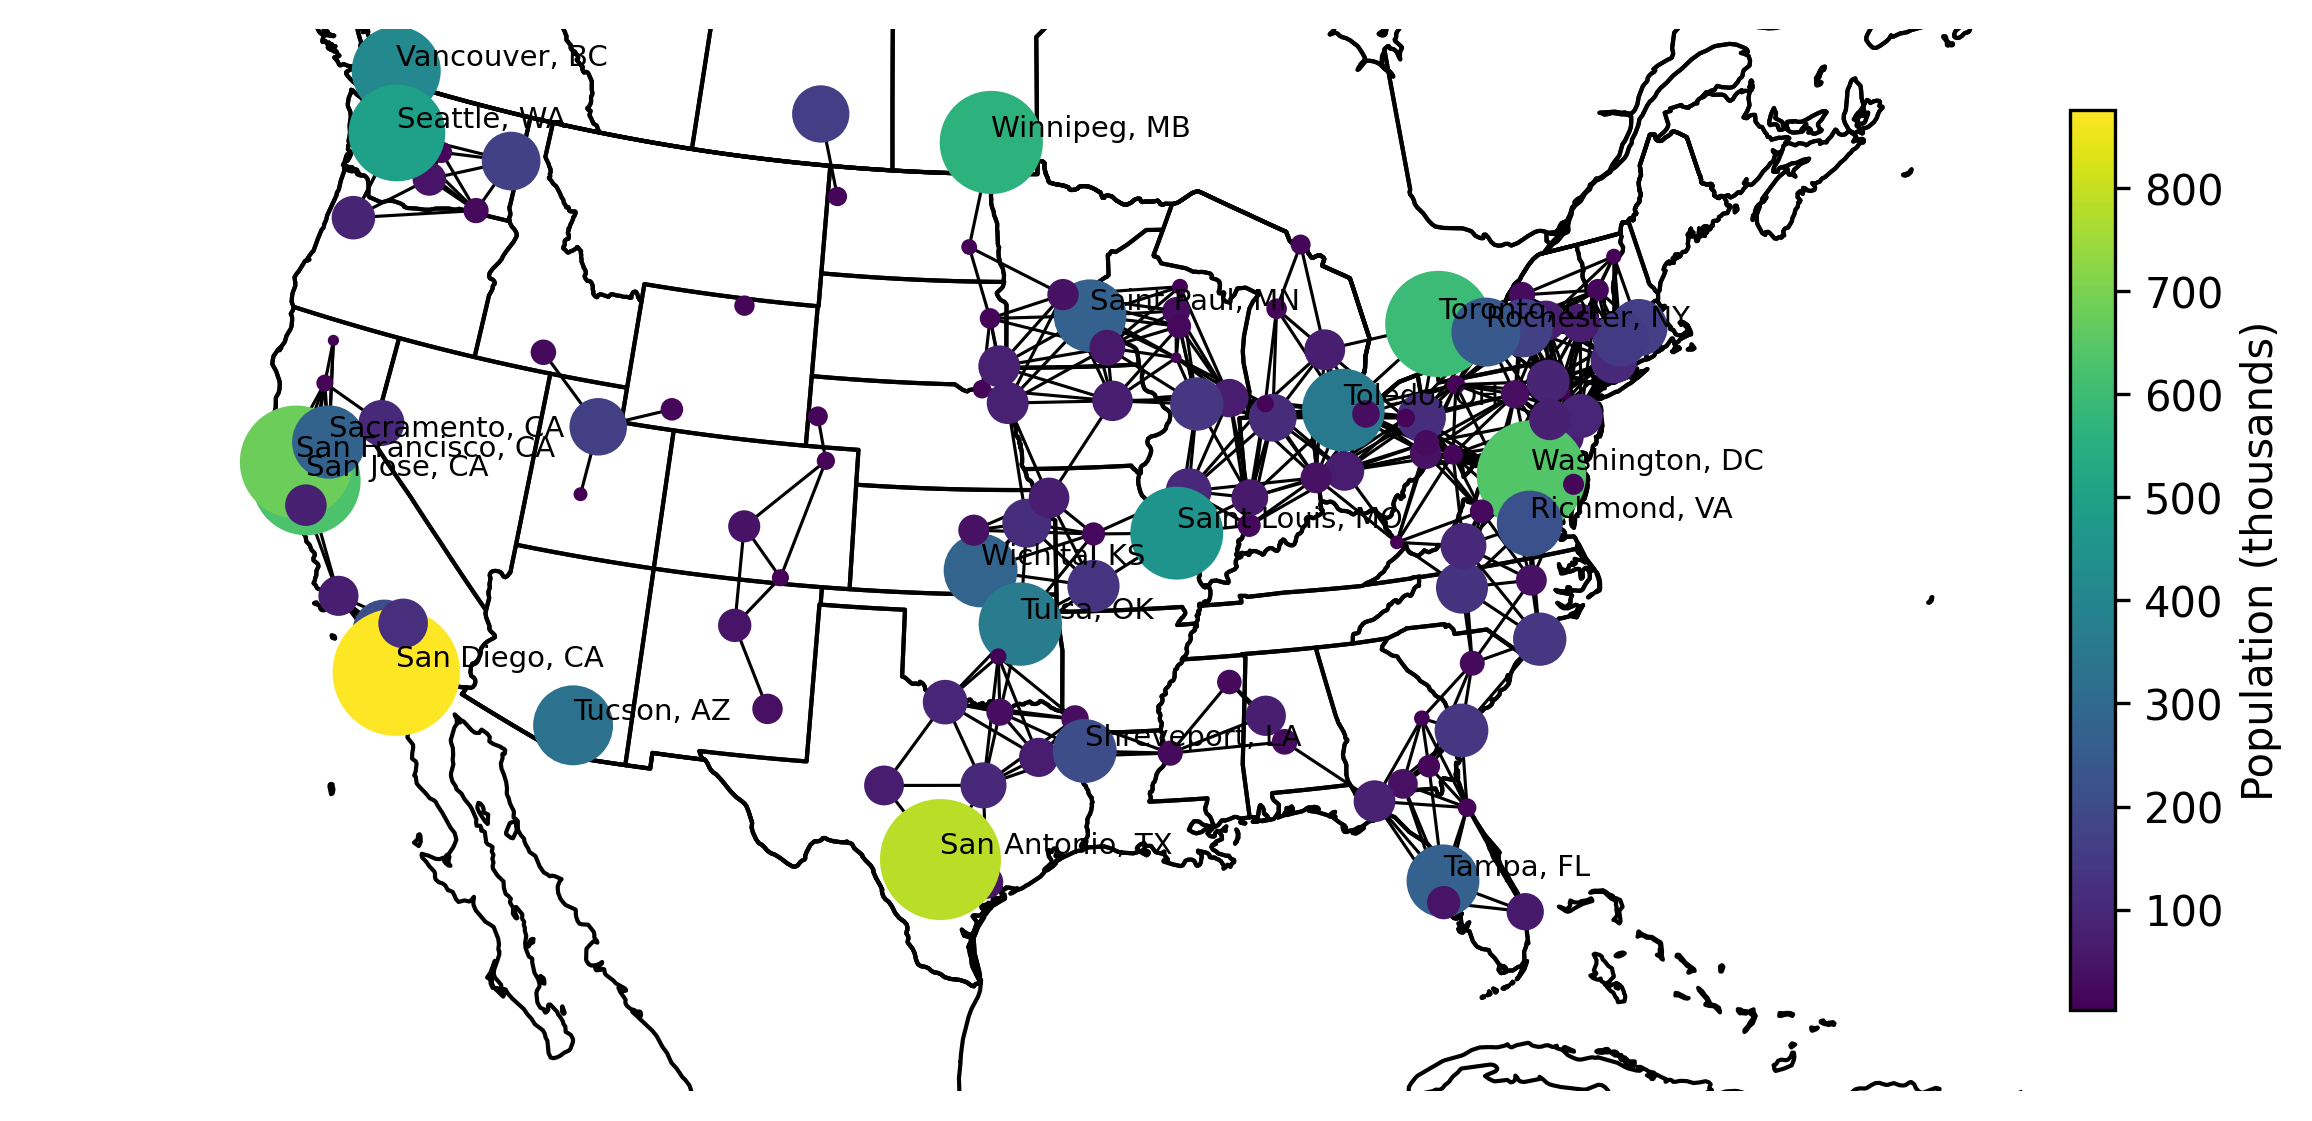
\includegraphics[width=0.8\textwidth]{figures/geographic_distribution.png}
    \caption{Geographic distribution of cities, with node size and color indicating population. Cities within 300 miles are connected.}
    \label{fig:geo_dist}
\end{figure}

\begin{itemize}
    \item Clear regional clustering of cities
    \item Population concentration in major metropolitan areas
    \item Natural geographical barriers affecting connectivity
    \item Dense network of connections in the eastern United States
\end{itemize}

\section{Population Analysis}
The population analysis reveals:
\begin{itemize}
    \item Mean population: 120,000
    \item Median population: 68,000
    \item Standard deviation: 167,000
    \item Range: 3,000 to 876,000
\end{itemize}

This indicates a right-skewed distribution typical of urban systems, with a few large cities and many smaller ones.

\subsection{Population Distribution Visualization}
Figure \ref{fig:pop_dist} shows the distribution of city populations:

\begin{figure}[H]
    \centering
    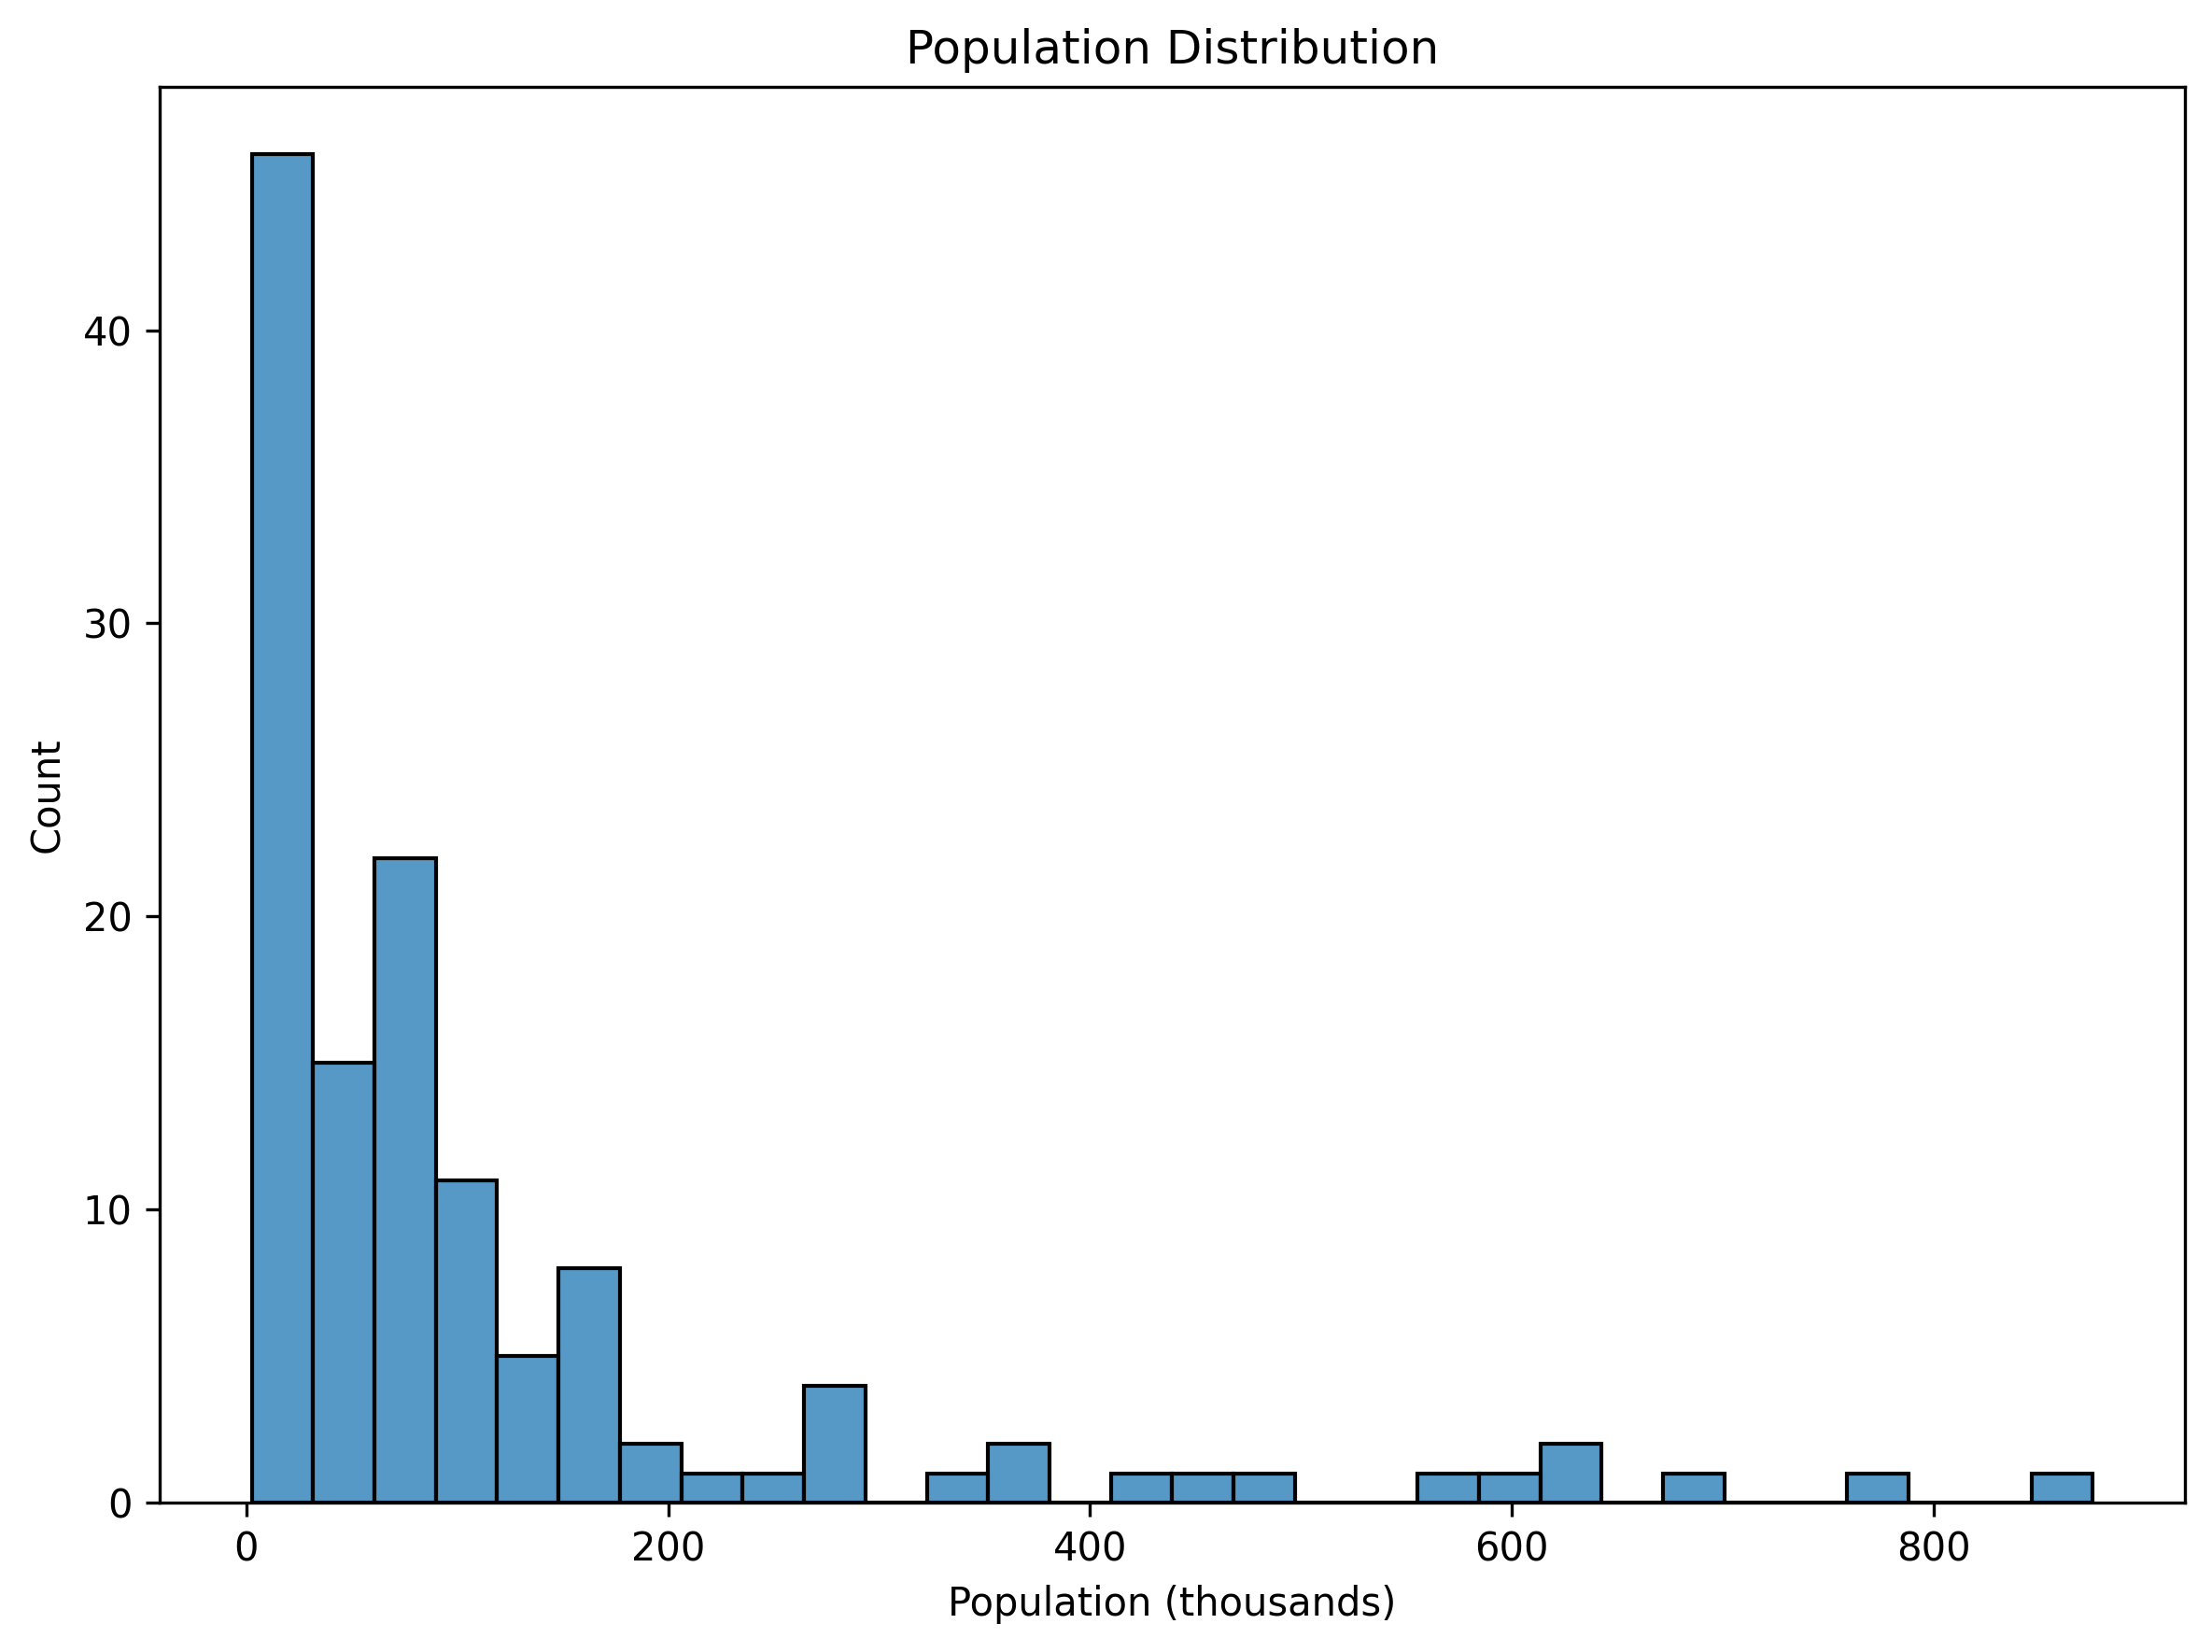
\includegraphics[width=0.8\textwidth]{figures/population_distribution.png}
    \caption{Distribution of city populations, showing the right-skewed nature of the data.}
    \label{fig:pop_dist}
\end{figure}

The histogram reveals:
\begin{itemize}
    \item Majority of cities have populations below 200,000
    \item Few cities with very large populations
    \item Clear right-skew in the distribution
    \item Natural breaks in the population distribution
\end{itemize}

\section{Distance Analysis}

\subsection{Longest Distances}
The analysis of longest city-to-city distances shows:
\begin{itemize}
    \item Cross-continental connections
    \item Maximum distances typically between cities on opposite coasts
    \item Geographical constraints influencing maximum distances
\end{itemize}

Figure \ref{fig:longest_dist} illustrates the top 10 longest city-to-city distances:

\begin{figure}[H]
    \centering
    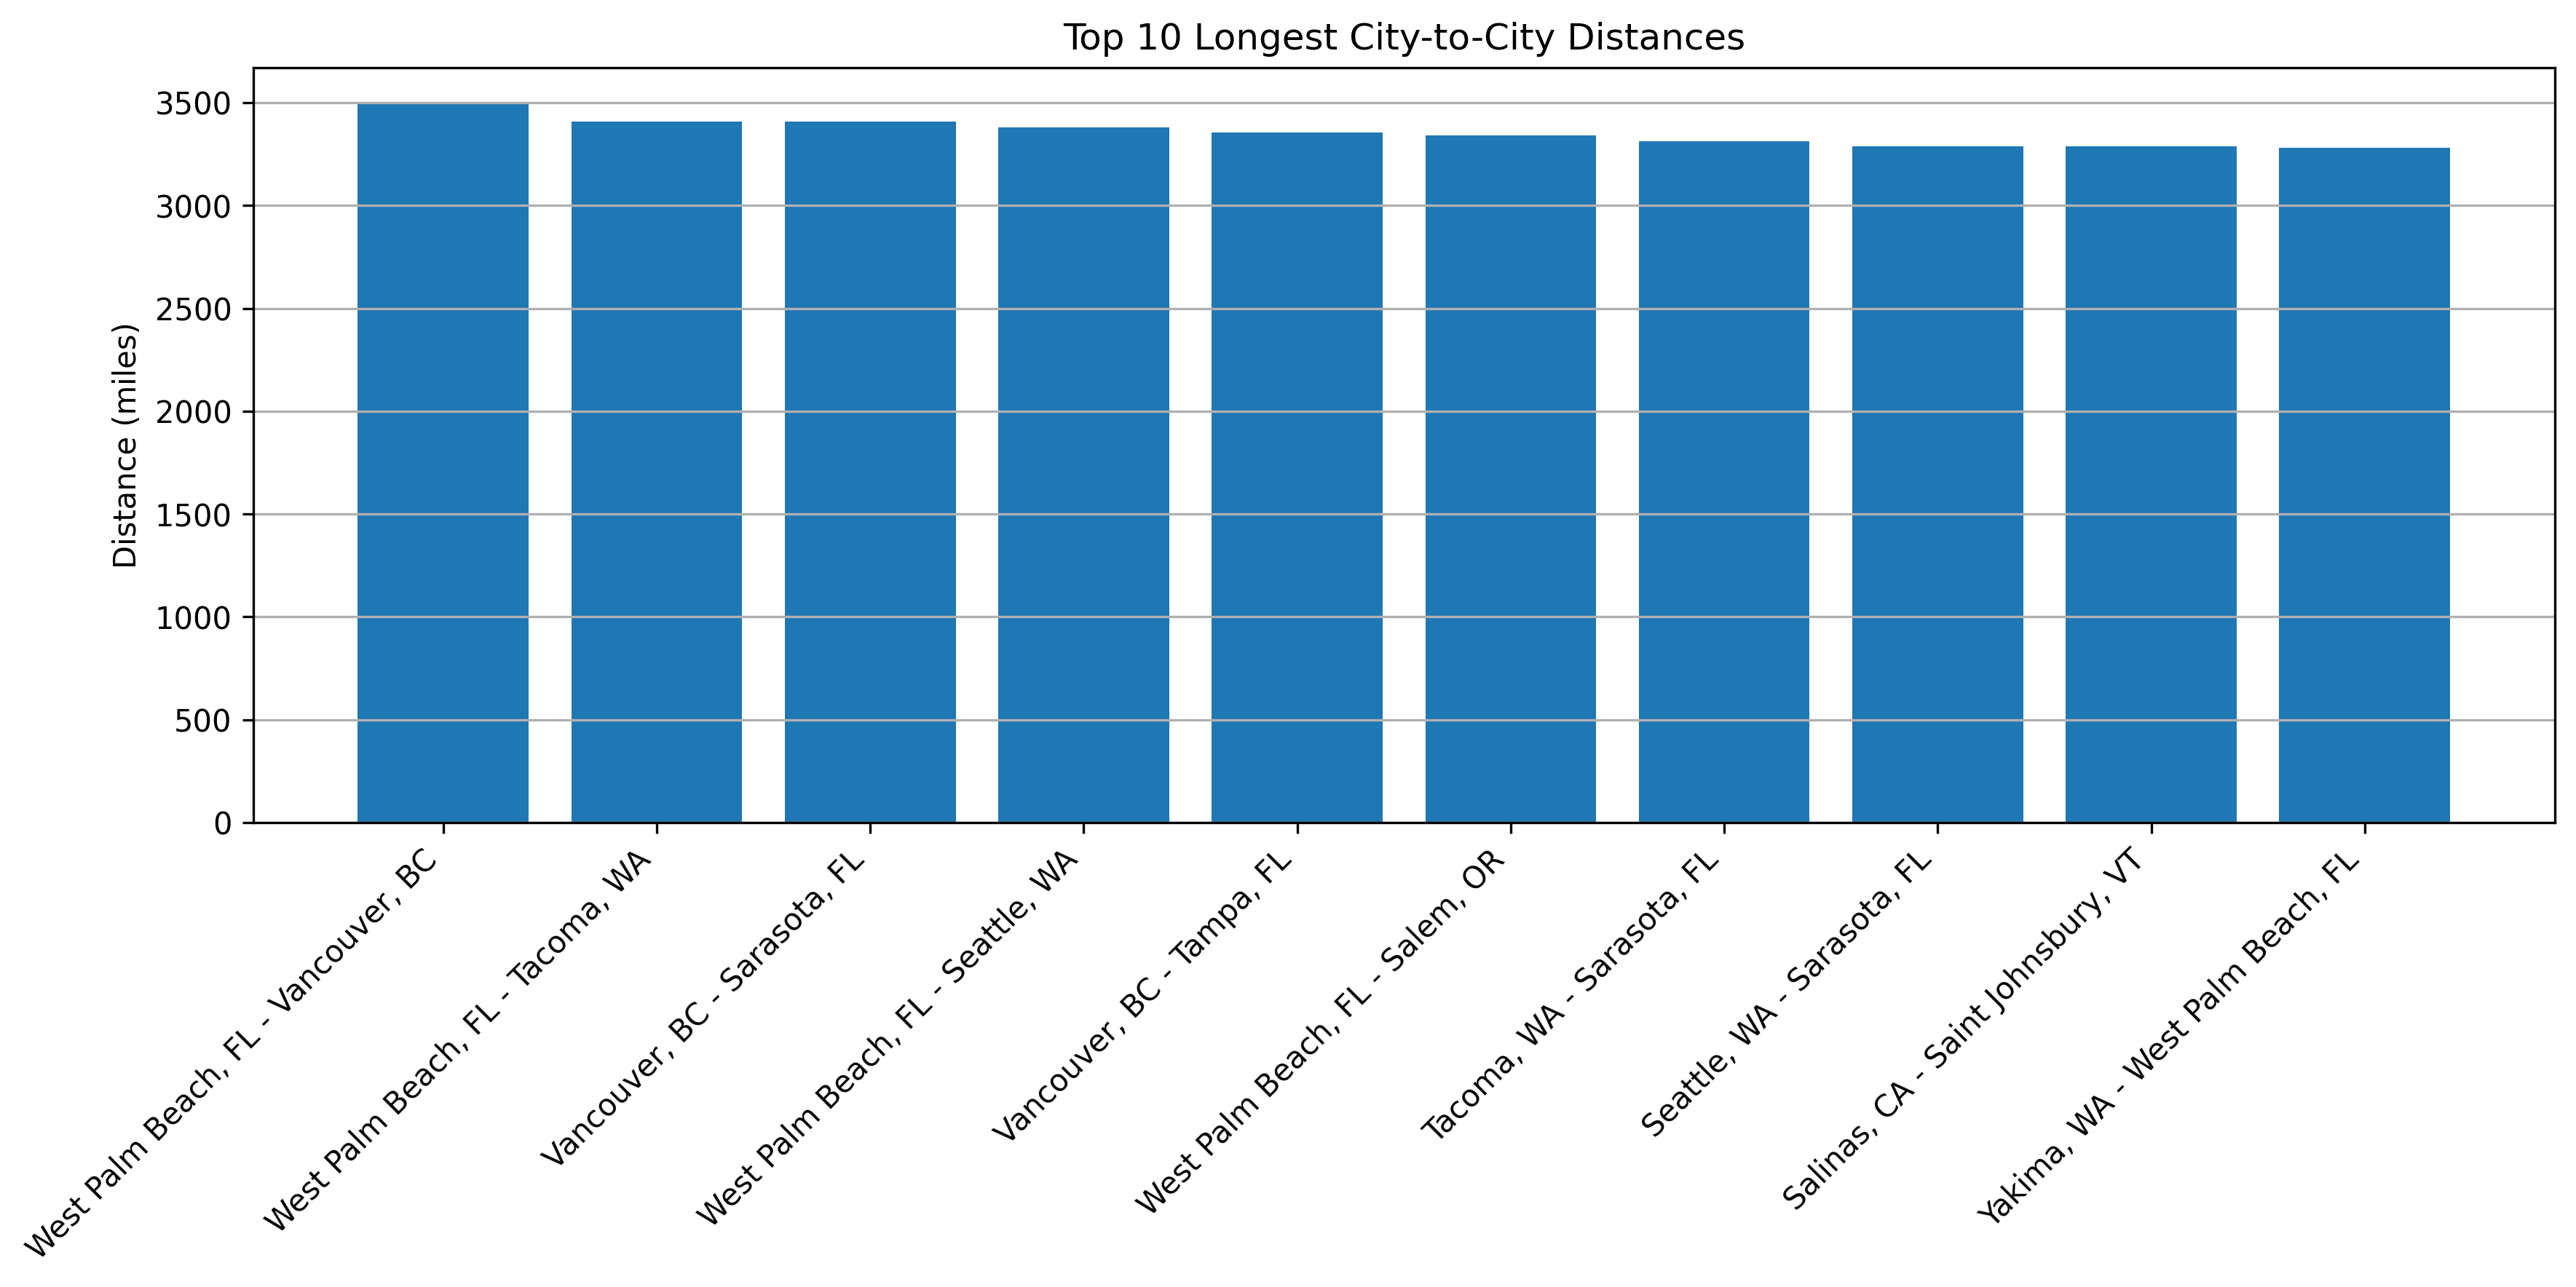
\includegraphics[width=0.8\textwidth]{figures/longest_distances.png}
    \caption{Top 10 longest city-to-city distances in the network.}
    \label{fig:longest_dist}
\end{figure}

Key observations:
\begin{itemize}
    \item Maximum distances exceed 3000 miles
    \item Most long distances involve cities on opposite coasts
    \item Clear geographical patterns in the longest connections
\end{itemize}

\subsection{Shortest Distances}
The shortest distances analysis reveals:
\begin{itemize}
    \item Clustering of cities in metropolitan areas
    \item Regional connectivity patterns
    \item Natural geographical proximity
\end{itemize}

Figure \ref{fig:shortest_dist} shows the top 10 shortest city-to-city distances:

\begin{figure}[H]
    \centering
    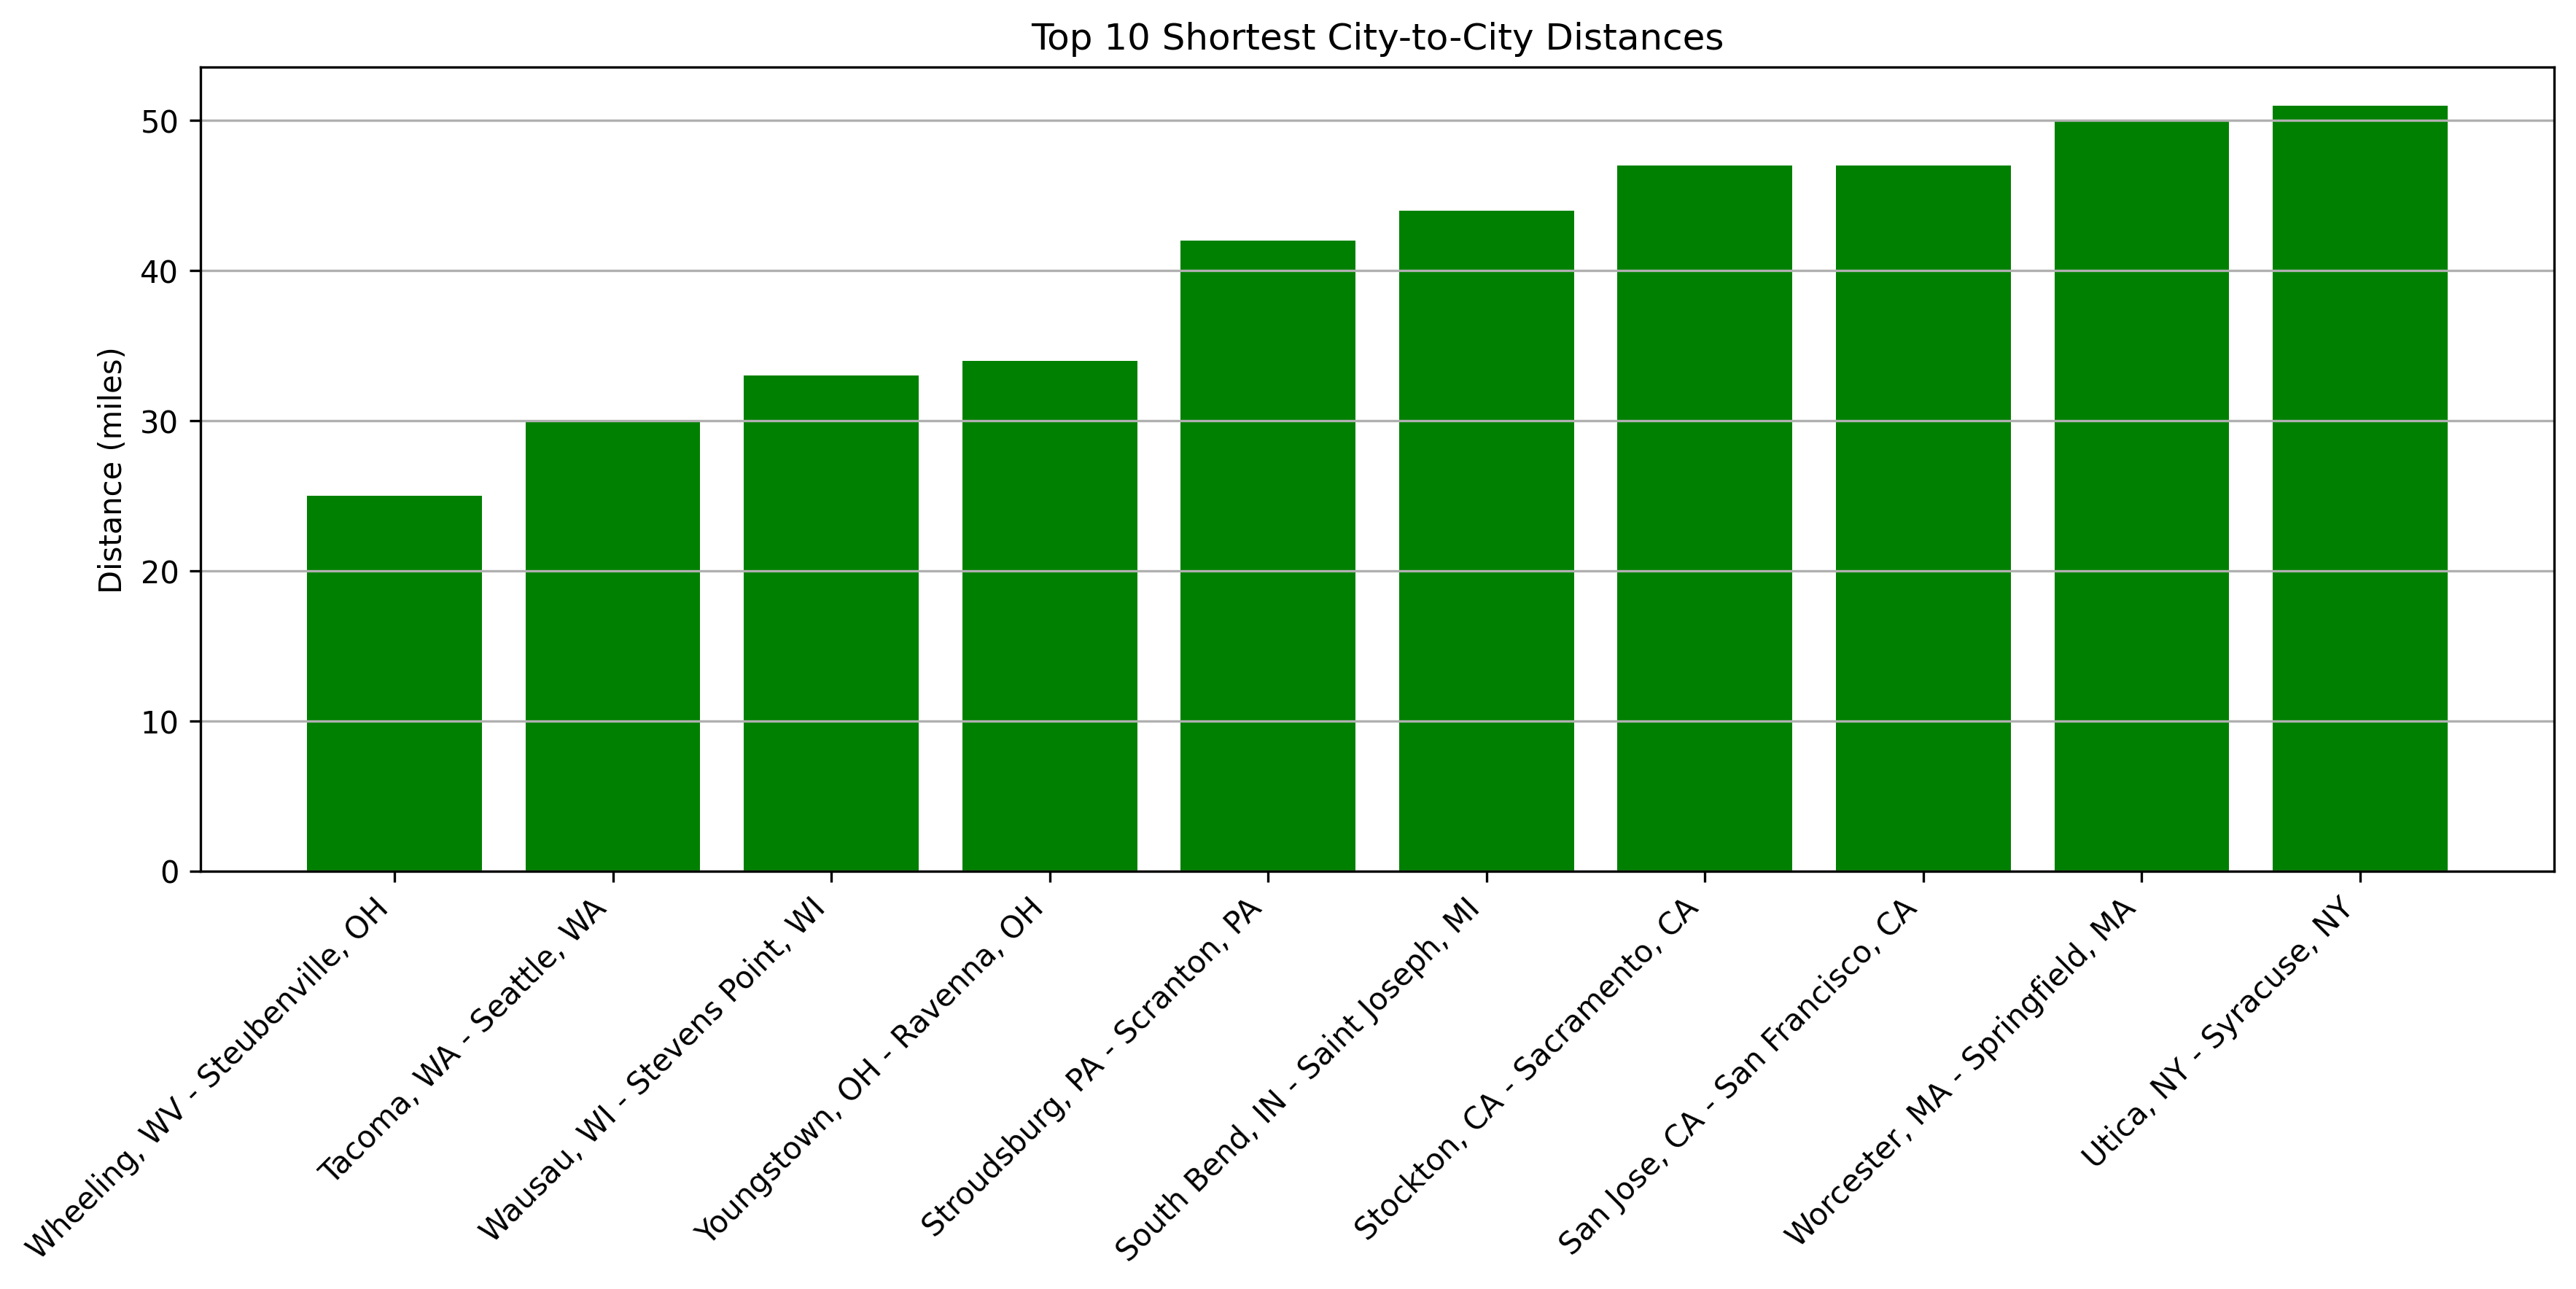
\includegraphics[width=0.8\textwidth]{figures/shortest_distances.png}
    \caption{Top 10 shortest city-to-city distances in the network.}
    \label{fig:shortest_dist}
\end{figure}

Key observations:
\begin{itemize}
    \item Shortest distances typically less than 50 miles
    \item Most short distances between cities in the same metropolitan area
    \item Clear regional clustering in the shortest connections
\end{itemize}

\section{Network Properties}
The complete graph structure of the network results in:
\begin{itemize}
    \item Network density: 1.0
    \item Average degree: 127
    \item Uniform degree distribution
    \item Weighted edges representing actual distances
\end{itemize}

\section{Visualization}
The network visualization using Cartopy reveals:
\begin{itemize}
    \item Spatial distribution of cities
    \item Population-based node sizing
    \item Distance-based edge weights
    \item Regional clustering patterns
\end{itemize}

These visualizations help in understanding the geographical context of the network and the relationships between cities. 